\subsection{Wagwoord herstel onderdeel}

Die wagwoord herstel onderdeel verskaf funksionaliteit vir gebruikers om
hul wagwoorde te herstel wanneer hulle dit vergeet het. Dit sluit 'n
veilige proses in wat e-pos verifikasie gebruik om wagwoord herstel
versoeke te hanteer en nuwe wagwoorde te stel.

\begin{figure}[H]
    \centering
    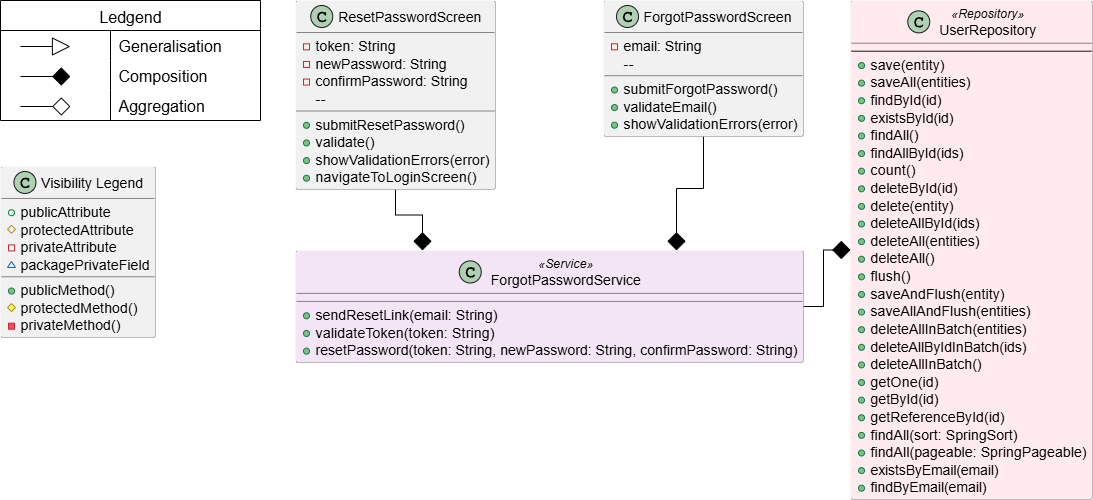
\includegraphics[width=\textwidth]{figures/class_diagrams/reset-password-subsystem.png}
    \caption{Wagwoord herstel onderdeel klasdiagram}
    \label{fig:reset_password_subsystem_class_diagram}
\end{figure}

Hier volg die CRC kaarte vir die belangrikste klasse in hierdie
onderdeel.

\vspace{1em}
\textbf{ResetPasswordScreen} bied die koppelvlak vir gebruikers om 'n nuwe wagwoord in te voer, te valideer en die herstelproses te bevestig.
\begin{table}[H]\centering\begin{tabular}{|p{0.4\textwidth}|p{0.4\textwidth}|}
    \hline
    \multicolumn{2}{|c|}{\textbf{ResetPasswordScreen}} \\
    \hline
    \textbf{Verantwoordelikhede} & \textbf{Medewerkers} \\
    \hline
    Verskaf vorm vir nuwe wagwoord invoer \newline
    Valideer wagwoord sterkte en ooreenstemming \newline
    Bevestig wagwoord herstel \newline
    Wys sukses of fout boodskappe
    &
    ForgotPasswordService \\
    \hline
\end{tabular}
\caption{CRC vir ResetPasswordScreen}
\label{tab:crc_reset_password_screen}
\end{table}

\vspace{1em}
\textbf{ForgotPasswordScreen} verskaf die vorm vir e-posinvoer, inisieer die herstelproses en valideer die e-posadres.
\begin{table}[H]\centering\begin{tabular}{|p{0.4\textwidth}|p{0.4\textwidth}|}
    \hline
    \multicolumn{2}{|c|}{\textbf{ForgotPasswordScreen}} \\
    \hline
    \textbf{Verantwoordelikhede} & \textbf{Medewerkers} \\
    \hline
    Verskaf vorm vir e-pos adres invoer \newline
    Inisieer wagwoord herstel proses \newline
    Valideer e-pos adres formaat \newline
    Wys bevestiging van herstel versoek
    &
    ForgotPasswordService \\
    \hline
\end{tabular}
\caption{CRC vir ForgotPasswordScreen}
\label{tab:crc_forgot_password_screen}
\end{table}

\vspace{1em}
\textbf{ForgotPasswordService} verwerk wagwoordherstelversoeke, genereer en valideer tokens, werk wagwoorde by en hanteer sekuriteit.
\begin{table}[H]\centering\begin{tabular}{|p{0.4\textwidth}|p{0.4\textwidth}|}
    \hline
    \multicolumn{2}{|c|}{\textbf{ForgotPasswordService}} \\
    \hline
    \textbf{Verantwoordelikhede} & \textbf{Medewerkers} \\
    \hline
    Verwerk wagwoord herstel versoeke \newline
    Genereer en stuur herstel tokens \newline
    Valideer herstel tokens \newline
    Werk gebruiker wagwoorde by \newline
    Hanteer token verval en sekuriteit
    &
    UserRepository \\
    \hline
\end{tabular}
\caption{CRC vir ForgotPasswordService}
\label{tab:crc_forgot_password_service}
\end{table}

\section{Slotopmerking}
Die databasisontwerp, \textit{sitemap}, \ac{CRC} kaarte en klasdiagramme vorm 'n
omvattende basis vir die stelsel se argitektuur en ontwerp. Hierdie elemente is
belangrik om die struktuur, funksionaliteit en interaksies van die stelsel duidelik te verstaan. Deur die visuele en beskrywende voorstellings wat in hierdie hoofstuk aangebied is, word die ontwikkeling, implementering en toekomstige uitbreiding van die stelsel vergemaklik. Die samehang tussen die databasis, gebruikerskoppelvlak en dienslaag word duidelik uiteengesit, wat nie net die implementering ondersteun nie, maar ook die instandhouding en skaalbaarheid van die stelsel in die toekoms verseker.